\documentclass{article}


% if you need to pass options to natbib, use, e.g.:
\PassOptionsToPackage{sort, numbers}{natbib}
% before loading neurips_2023


% ready for submission
% \usepackage{neurips_2023}


% to compile a preprint version, e.g., for submission to arXiv, add add the
% [preprint] option:
%     \usepackage[preprint]{neurips_2023}


% to compile a camera-ready version, add the [final] option, e.g.:
\usepackage[final]{neurips_2023}


% to avoid loading the natbib package, add option nonatbib:
%    \usepackage[nonatbib]{neurips_2023}


\usepackage[utf8]{inputenc} % allow utf-8 input
\usepackage[T1]{fontenc}    % use 8-bit T1 fonts
\usepackage{hyperref}       % hyperlinks
\usepackage{url}            % simple URL typesetting
\usepackage{booktabs}       % professional-quality tables
\usepackage{amsfonts}       % blackboard math symbols
\usepackage{amsmath}
\usepackage{amssymb}
\usepackage{nicefrac}       % compact symbols for 1/2, etc.
\usepackage{microtype}      % microtypography
\usepackage{xcolor}         % colors
\usepackage{xspace}         % space after command
\usepackage{graphicx}
\usepackage{subcaption}
\usepackage{bm}
\usepackage{physics}
\usepackage[capitalize]{cleveref}       % smart references
\usepackage{multirow}
\usepackage{minted}
\usepackage[font=small]{caption}
\usepackage[nolist]{acronym}  % acronyms
\usepackage{tikz}  % draw board
\usepackage{adjustbox}  % centering tikz in table

\bibliographystyle{plainnat}

\newcommand{\todo}[1]{\textcolor{red}{TODO: #1}}
\newcommand{\ttgpt}{TicTacGPT\xspace}
\newcommand{\ttt}{Tic-Tac-Toe\xspace}

\renewcommand{\v}[1]{\mathbf{\bm{#1}}}
\newcommand{\m}[1]{\mathbf{\bm{#1}}}
\newcommand{\I}{\m{I}}
\newcommand{\R}{\mathbb{R}}
\DeclareMathOperator{\softmax}{Softmax}
\DeclareMathOperator{\solu}{SoLU}
\DeclareMathOperator{\layernorm}{LN}
\DeclareMathOperator{\tril}{Tril}
\DeclareMathOperator{\attn}{Attn}

\newcounter{num}
\newcommand{\tictactoe}[1]{
\begin{tikzpicture}[scale=0.4]
    \def\r{1.4mm}
    \tikzset{
        circ/.pic={\draw circle (\r);},
        cross/.pic={\draw (-\r,-\r) -- (\r,\r) (-\r,\r) -- (\r,-\r);},
    }
        
    % The grid
    \foreach \i in {0,1,2,3} \draw (\i,0) -- (\i,3) (0,\i) -- (3,\i);
    
    % Numbering the cells
    \setcounter{num}{0}
    \foreach \y in {0,...,2}
        \foreach \x in {0,...,2}
            {
            \coordinate (\thenum) at (\x+0.5,2-\y+0.5);
            %\node[opacity=0.5] at (\thenum) {\sffamily\thenum}; % Uncomment to see numbers in the cells
            \addtocounter{num}{1}
            }
                
                
    \def\X{X} \def\O{O} \def\n{n}
    
    \foreach \l [count = \i from 0] in {#1}
        {
        \if\l\X \path (\i) pic{cross};
        \else\if\l\O \path (\i) pic{circ};
        \else\if\l\n \node[opacity=0.5] at (\i) {\sffamily\i};
        \fi
        \fi
        \fi
        }
\end{tikzpicture}
}
\newcommand{\cbox}[1]{\adjustbox{valign=c}{#1}}


\hypersetup{
    colorlinks,
    linkcolor={red!50!black},
    citecolor={blue!50!black},
    urlcolor={black}
}

\title{Fully Understanding a Sequence Model of Tic-Tac-Toe}

\author{%
  Andy Lo \\
  Department of Computer Science\\
  University of Cambridge\\
  \texttt{cyal4@cam.ac.uk} \\
}


\begin{document}

\begin{acronym}
    \acro{LLMs}{Large Language Models}
\end{acronym}


\maketitle


\begin{abstract}
    While \ac{LLMs} demonstrate strong capabilities from simple sequence modelling, its inner workings remain as a black-box. In this project, as a step towards interpreting \ac{LLMs}, I fully reverse engineer a toy sequence model trained on \ttt game sequences. \todo{Add results}
\end{abstract}


\section{Introduction}

While the success of deep learning in practice is ubiquitous, interpreting and explaining the behaviour of neural networks remain a difficult problem. The inability to understand the models' internal components is a significant bottleneck to building reliable machine learning systems since typical evaluation methods provides no guarantee when given out-of-distribution inputs. Mechanistic interpretability is an emerging approach to explainability by focusing on tractable, low-level components of a model, using them as an entry point to build an overall understanding of a model's behaviour. This project aims to build upon this line of work, showcasing another example where models are not black boxes and can be made human-interpretable with sufficient effort. \todo{Add citations}

There has been particular interest in understanding sequence models trained with next-token prediction, specifically on whether next-token prediction is sufficient for building generally intelligent models. On one hand, there exists theoretical arguments \citep{bender2020climbing,merrill2021provable} that such models merely learn statistical correlations and thus cannot understand the casual relationships of the underlying data generation process. On the other hand, many empirical studies reveal opposing evidence where models appear to have build accurate world models internally. Unfortunately, models used in practice are often too complex to be understood \emph{fully} as they are often too large and many factors like data selection and training optimisations are not controlled for. Several works have thus shifted its focus to simpler sequence models on synthetic datasets \citep{toshniwal2021learning,orthello-gpt} where the task is well-understood.

This project studies sequence models trained on synthetic game sequences of \ttt. The simplistic nature of the task permits the use of a one-layer transformer that still solves the task perfectly. This greatly simplifies the analysis and allows us to fully reverse engineer the model, resulting in predictable behaviour even on out-of-distribution data. \todo{Explain contributions.}

\section{Background}

This section covers the necessary background to understand the contributions of this project. \cref{sec:related} provides an overview of the most relevant works and how they relate to this project. \cref{sec:math} describes the framework and the notation used later in this paper to describe components of a transformer.

\subsection{Related works} \label{sec:related}

\citet{toshniwal2021learning} were the first to probe for internal world presentations of next-token prediction models. The authors reveal that models trained to predict the next moves in chess track the state of the board internally. \citet{orthello-gpt} extend this idea by studying a next-move prediction model trained on Orthello. They demonstrate that not only do the models track the board state, interventions on the internal representation also have the expected casual effect on the model's outputs. This provides strong evidence that models trained on sequence modelling can in fact ``understand'' the nature of the task rather than simply memorising statistical patterns. \citet{linear-orthello-gpt} further reveal that the board state can be expressed as a linear projection of the internal representation. While such works identify core properties of the model like its internal representations, they still fail to explain the model behaviour in full. For example, no explanation is offered as to \emph{how} the internal board representations are computed. This project aims to close this gap by narrowing the focus to even simpler tasks and models.

\todo{Talk about other MI works}

\subsection{Mathematical framework of transformers} \label{sec:math}

To conveniently reason about various components of the transformer \citep{vaswani2017attention}, it is helpful to set up a mathematical description of it \citep{elhage2021mathematical}. While the following description maybe verbose, several simplifications can be made when combined with empirical evidence (\cref{sec:simplify}). The notation will only cover one-layer transformers since that is the main focus of this project.

Let $\m{E} \in \R^{s \times v}$ be the one-hot encoded input tokens, where $s$ is the sequence length and $v$ is the vocabulary size. The embedding layer with learnt positional embeddings can be expressed as:
\begin{equation}  \label{eq:embed}
    \text{Embed}(\m{E}) = \m{E} \m{W}_E + \m{W}_P
\end{equation}
where $\m{W}_E \in \R^{v \times d}$, $\m{W}_P \in \R^{s \times d}$ and $d$ is the hidden dimension of the model.

The core component of the transformer is the attention layer. In this project, we focus on the multi-head, casual, self-attention variant. Each attention head $i$ is parameterised by the query $\m{W}_Q^{(i)} \in \R^{d \times h}$, $\v{b}_Q^{(i)} \in \R^{1 \times h}$, key $\m{W}_K^{(i)} \in \R^{d \times h}$, $\v{b}_K^{(i)} \in \R^{1 \times h}$, value $\m{W}_V^{(i)} \in \R^{d \times h}$, $\v{b}_V^{(i)} \in \R^{1 \times h}$ and output $\m{W}_O^{(i)} \in \R^{h \times d}$, $\v{b}_O^{(i)} \in \R^{1 \times d}$ projections, where $h$ is the head dimension. The attention operator can be expressed as:
\begin{equation}  \label{eq:attn}
    \begin{aligned}
        \attn(\m{X})
         & = \sum_i \m{A}^{(i)} (\m{X} \m{W}_V^{(i)} + \v{1}_s \v{b}_V^{(i)}) \m{W}_O^{(i)} + \v{1}_s \v{b}_O^{(i)} \\
        \m{A}^{(i)}
         & = \softmax\left(
        \tril\left(
        \left(\m{X} \m{W}_Q^{(i)} + \v{1}_s \v{b}_Q^{(i)}\right)
        \left(\m{X} \m{W}_K^{(i)} + \v{1}_s \v{b}_K^{(i)}\right)^T
        , -\infty\right)
        \right)
    \end{aligned}
\end{equation}
where $\v{1}_s \in \R^{s \times 1}$ is a vector of ones and $\tril(\m{X}, y)$ fills the upper triangular matrix of $\m{X}$ with $y$. The typical scaling by factor of $1/\sqrt{d}$ in the attention matrix is ignored as it is a linear operation and thus can be folded into the weights.

The other building block is the MLP block which can be expressed as:
\begin{equation*}
    \text{MLP}(\m{X}) = \phi(
    \m{X} \m{W}_{in} + \v{1}_s \m{b}_{in}
    ) \m{W}_{out} + \v{1}_s \m{b}_{out}
\end{equation*}
where $\m{W}_{in} \in \R^{d \times 4d}$, $\v{b}_{in} \in \R^{1 \times 4d}$, $\m{W}_{out} \in \R^{4d \times d}$, $\v{b}_{out} \in \R^{1 \times d}$ and $\phi$ is an elementwise non-linearity.

Putting everything together, the transformer output $\m{Y} \in \R^{s \times v}$ can be expressed as:
\begin{equation}  \label{eq:transformer}
    \begin{aligned}
        \m{H}_0 & = \text{Embed}(\m{E})                           \\
        \m{H}_1 & = \m{H}_0 + \attn(\layernorm(\m{H}_0))          \\
        \m{H}_2 & = \m{H}_1 + \text{MLP}(\layernorm(\m{H}_1))     \\
        \m{Y}   & = \layernorm(\m{H_2}) \m{W}_U + \v{1}_s \v{b}_U
    \end{aligned}
\end{equation}
where $\m{W}_U \in \R^{d \times v}$, $\v{b}_U \in \R ^{1 \times v}$ and $\layernorm(\m{X})$ represents a LayerNorm which normalises $\m{X}$ column-wise by subtracting the mean and dividing by the standard deviation. The scale and bias parameters of LayerNorm is ignored as they can be folded into the linear projections that proceed them.

\section{\ttgpt}

\subsection{Synthetic task and dataset}

\begin{figure}
    \centering
    \renewcommand{\arraystretch}{1.3}
    \begin{tabular}{lccccccc}
        Game
         & \cbox{\tictactoe{
                n,n,n,
                n,n,n,
                n,n,n,
            }}
         & \cbox{\tictactoe{
                _,X,_,
                _,_,_,
                _,_,_,
            }}
         & \cbox{\tictactoe{
                _,X,_,
                _,O,_,
                _,_,_,
            }}
         & \cbox{\tictactoe{
                _,X,_,
                _,O,_,
                _,_,X,
            }}
         & \cbox{\tictactoe{
                _,X,_,
                _,O,O,
                _,_,X,
            }}
         & \cbox{\tictactoe{
                X,X,_,
                _,O,O,
                _,_,X,
            }}
         & \cbox{\tictactoe{
                X,X,_,
                O,O,O,
                _,_,X,
        }}                   \\
        \midrule
        Input
         & \texttt{[B]}
         & \texttt{1}
         & \texttt{4}
         & \texttt{8}
         & \texttt{5}
         & \texttt{0}
         & \texttt{3}        \\
        Target
         & \texttt{1}
         & \texttt{4}
         & \texttt{8}
         & \texttt{5}
         & \texttt{0}
         & \texttt{3}
         & \texttt{[O]}      \\
    \end{tabular}
    \caption{Example of a \ttt game and its corresponding inputs and next-token prediction targets. The numbering of the board positions are shown in the first board (top left). \texttt{[B]} is the special beginning-of-sequence token and \texttt{[O]} denotes the end of the game with the result ``\texttt{O} wins''.}
    \label{fig:game-sample}
\end{figure}

Following \cite{orthello-gpt}, each game is represented as the sequence of moves played, where each move of the 9 possible moves are encoded as a separate token. The special beginning-of-sequence token \texttt{[B]} is prepended to every game sequence. A result token also is appended, it is one of \texttt{[X]}, \texttt{[O]} or \texttt{[D]}, representing ``\texttt{X} wins'', ``\texttt{O} wins'' and ``Draw'' respectively. An example of an encoded game is shown in \cref{fig:game-sample}. Ignoring rotational and reflectional symmetries there are 255,168 unique games of \ttt. The train and test dataset is constructed by randomly splitting all the games into two set of equal size.

One might naively think that the task only involves learning what moves are legal and deciding the final outcome of the game. However, there are nuances to the training objective. Since the model is trained on all possible game sequences, the true task is to learn the proportion of possible continuations for each possible next move. For example, the optimal model should assign lower probability to immediately winning moves (one that creates a three-in-a-row) as there is only one continuation (either ``\texttt{X} wins'' or ``\texttt{O} wins'') while non-winning moves have more possible continuations. As shown later, the trained model captures such complexities of the task as well.

\subsection{Model and experiment details}

The training of \ttgpt mostly follows standard practices \citep{radford2019language} for typical prefix \ac{LLMs}. \ttgpt is a one-layer transformer with 128 hidden dimensions, 2 attention heads, 512 MLP dimensions, learnt positional encodings and uses the pre-norm architecture \citep{xiong2020layer}. The only non-standard architectural choice is the use of the Softmax Linear Units ($\solu$) \citep{elhage2022solu} activation function in the MLP. It is defined as:
\begin{equation*}
    \solu(\m{X}) = \layernorm(\m{X} \cdot \softmax(\m{X}))
\end{equation*}
\citet{elhage2022solu} demonstrated that $\solu$ increases the interpretability of MLP neurons such as by reducing polysemanticity\footnote{Polysemanticity is the phenomenon where neurons respond to multiple unrelated inputs.}\citep{olah2020zoom} while having negligible impact on performance. Empirically I found that models trained with $\solu$ produced slightly ``cleaner'' activation patterns than standard choices like $\text{GeLU}$ though the effect is not substantial. The model is trained for 40000 steps with batch size 512 using the AdamW optimizer \citep{loshchilov2017decoupled} with learning rate $0.0003$, $\beta_1 = 0.9$, $\beta_2 = 0.999$ and weight decay $0.1$ on non-bias and non-embedding parameters.

\section{Three simplifying properties} \label{sec:simplify}

\begin{table}
    \caption{A one-layer transformer solves the \ttt task optimally. KL div. is the KL divergence between the optimal distribution and that predicted by the model, averaged across all game sequences. Legal move acc. measures whether the top-predicted move is a legal move, averaged across all \emph{prefixes}. Top move acc. measures whether the top-predicted move is also (one of) the top move(s) under the optimal model, averaged across all prefixes.}
    \label{table:eval}
    \centering
    \begin{tabular}{llll}
         & KL div. (nats)
         & Legal move acc. (\%)
         & Top move acc. (\%)   \\
        \toprule
        \ttgpt
         & \textbf{0.0042}
         & \textbf{100}
         & \textbf{99.56}       \\
        Two-layer transformer
         & 0.0060
         & 99.88
         & 99.33                \\
        Chance level
         & 1.0664
         & 13.58
         & 11.25                \\
        \midrule
        \ttgpt (MLP only)
         & 0.0105
         & 100
         & 98.73
    \end{tabular}
\end{table}

This section lays down and provides empirical evidence to several appealing properties of the trained model that make it particularly friendly to mechanistic analysis. The remainder of this report will base its argument on such simplifications.

\subsection{\ttgpt solves \ttt}

The first observation is that a one-layer transformer is sufficient to solve the task almost optimally. One of the advantages of working with a toy problem like \ttt is that the optimal policy can be computed exactly, by enumerating all game sequences. This makes evaluation much simpler as we can directly compare the trained models to the optimal model. \cref{table:eval} shows such comparisons with the optimal model for \ttgpt, a two-layer counterpart\footnote{The two-layer model uses the same hyperparameters, except having two layers and is trained with a lower weight decay of 0.03 (as it failed to converge with weight decay 0.1).} and a baseline constant output model. \ttgpt achieves much better performance than random and approaches 100\% accuracy on other classification metrics. Surprisingly, it even outperforms the two-layer transformer which may be attributed to reduced overfitting. I thereby conclude that \ttgpt solves \ttt and thus the investigation of \emph{``How does a sequence model solve \ttt?''} can be limited to \emph{``How does \ttgpt solve \ttt?''}.

\subsection{Attention is only a function of position} \label{sec:simplify-attn}

\begin{figure}[t]
    \centering
    \begin{subfigure}[t]{0.55\textwidth}
        \includegraphics[width=\linewidth]{../out/figs/attn_pattern.pdf}
        \caption{A sample attention pattern of \ttgpt. Other inputs generally have the same pattern too.}
        \label{fig:attn-pattern}
    \end{subfigure}%
    \hfill
    \begin{subfigure}[t]{0.42\textwidth}
        \includegraphics[width=\linewidth]{../out/figs/sobol.pdf}
        \caption{Sobol decomposition of the unnormalised attention logits. Most of the variance can be explained by second order interactions between positional embeddings.}
        \label{fig:attn-sobol}
    \end{subfigure}
    \caption{The attention patterns of \ttgpt is approximately constant.}
    \label{fig:attn}
\end{figure}

The second observation is that the model appears to have learnt attention patterns that is independent of the input sequence. From the example attention map in \cref{fig:attn-pattern}, we see that both attention heads use checkerboard-like attention patterns. Heuristically, it appears that \texttt{Head0} is performing ``attend to all moves played by the opponent'' and \texttt{Head1} is doing the same but for the current player. Since the player order in \ttt is always the same (alternates between \texttt{X} and \texttt{O}), it is very likely that the attention pattern is derived from positional information alone.

To confirm the above intuition analytically, I perform sensitivity analysis of the attention pattern to identify which inputs have the most affect. To do so, I study a function $a^{(i)}$ that calculates the unnormalised attention paid by token $t_q$ at position $p_q$ on another token $t_k$ at position $p_k$, for attention head $i$. This can be done by unfolding the embedding and attention calculation as described by \cref{eq:embed,eq:attn}, giving the following definition:
\begin{equation*}
    \begin{aligned}
        a^{(i)}(t_q, p_q, t_k, p_k)
         & =\begin{cases}
                \left(\v{x}_q \m{W}_Q^{(i)} + \v{b}_Q^{(i)}\right)
                \left(\v{x}_k \m{W}_K^{(i)} + \v{b}_K^{(i)}\right)^T
                  & \text{if }p_k \leq p_q, \\
                0 & \text{otherwise.}
            \end{cases} \\
        \v{x}_q
         & = \layernorm((\m{W}_E)_{t_q} + (\m{W}_P)_{p_q})^T    \\
        \v{x}_k
         & = \layernorm((\m{W}_E)_{t_k} + (\m{W}_P)_{p_k})^T
    \end{aligned}
\end{equation*}
Treating $t_q, p_q, t_k, p_k$ as independent, uniformly distributed random variables, one can decompose the variance of $a^{(i)}$ into those explained by first-order terms (i.e. each input individually), second-order terms (i.e. interactions between pairs of inputs) and higher-order terms using Sobol's method \citep{sobol1993sensitivity,sobol2001global}. As shown in \cref{fig:attn-sobol}, nearly all of the variance can be explained by second-order interactions between $p_1$ and $p_2$. This matches our intuition since checkerboard attention patterns requires second-order interactions yet are purely positional. Thus, \ttgpt uses attention patterns that are input-independent and so \emph{the attention matrices $\m{A}^{(0)}, \m{A}^{(1)}$ are constants}.

\todo{Maybe characterise what the attention does here?}

\subsection{Output is only a function of MLP activations} \label{sec:simplify-output}

The last observation is that the skip connection around the MLP layer has minimal effect on the output logits, and thus can be ignored in our subsequent analysis. This property can be shown empirically by artificially removing the skip connection during inference (i.e. setting $\m{H}_2 = \text{MLP}(\layernorm(\m{H}_1))$) and studying its effects on the performance of the model. The comparison shown in \cref{table:eval} confirms such assertion, as the top move accuracy of the modified network only drops by $0.83\%$ and remains significantly better than chance.

The insignificance of the MLP skip connection means that we can narrow down the analysis to the MLP activations only. If we can understand how the MLP neurons respond to inputs and their corresponding effects on the output logits, we can explain most of the behaviour of \ttgpt.

\section{Zooming in: MLP neurons}

Given the simplifications from \cref{sec:simplify}, this section dives into the two circuits around the MLP layer that define the model's behaviour: The ``input circuit'' --- how do the MLP neurons respond to inputs, and the ``output circuit'' -- how do the activated neurons affect the output logits. The analysis will be done in two steps. Firstly, \cref{sec:neurons-that-matter} identifies the neurons that contribute the most to the model's performance. In the process, I discover that most of the behaviour can be explained by a small subset of neurons. Then, \cref{sec:neurons-visualisation} characterises the role of each of such neuron on the behaviour of the model.

\subsection{Neurons that matter} \label{sec:neurons-that-matter}

\begin{figure}[t]
    \centering
    \begin{subfigure}[t]{0.46\textwidth}
        \includegraphics[width=\linewidth]{../out/figs/neuron_importance.pdf}
        \caption{Effect of removing each neuron on the KL divergence, ordered from lowest to highest. Notice the y-axis is in log-scale.}
        \label{fig:neuron-importance}
    \end{subfigure}%
    \hfill
    \begin{subfigure}[t]{0.50\textwidth}
        \includegraphics[width=\linewidth]{../out/figs/neuron_pruning.pdf}
        \caption{The retained performance of pruning the bottom $n\%$ of neurons, ordered according to \cref{fig:neuron-importance}. The dotted line marks the 70\% threshold where there appears to be a clear cut-off.}
        \label{fig:neuron-pruning}
    \end{subfigure}
    \caption{Approximately 30\% of the neurons explain most of the performance of \ttgpt.}
    \label{fig:neurons}
\end{figure}

\ttgpt has 512 MLP neurons, which even in this toy problem is too many to be human comprehensible. To proceed, it is necessary to narrow down the number of MLP neurons for in-depth analysis.

However, identifying which neurons are the most ``important'' is non-trivial task. A naive approach might measure how often a neuron is ``active'' (e.g., larger than some threshold) across a diverse sample of game sequences. Unfortunately, this neglects the importance of neurons that only fire in response to particular inputs yet has a strong influence on the output logits. Another method might be to identify the neurons with the largest output logits influence by linearising the output circuit $(\m{W}_{out} + \v{1}_s \v{b}_{out}) \m{W_U}$. This however assumes each neuron fires with equal probability and equal magnitude, which is not guaranteed. For example, some neurons might never fire at all yet appear to have a large effect according to the output circuit.

Instead, I propose to take an empirical approach to measure neuron importance. To measure the significance of neuron $n$, I evaluate the performance of a patched version of \ttgpt where neuron $n$ is removed entirely. Concretely, the importance of a neuron is given by the increase in KL divergence from the optimal model of the patched model verses the original model, evaluated on a sample of 4096 games. The method is inspired by activation patching \citep{meng2022locating,vig2020investigating} which is commonly used to identify core components of a network.

\cref{fig:neuron-importance} shows that only a small proportion of neurons have a significant impact on the model's performance. Speculatively, this might be attributed to the use of SoLU non-linearity and weight decay which promotes sparse activations. To further quantify how many neurons can be ignored while still capturing most of the model's behaviour, I evaluate pruned versions of \ttgpt where $n\%$ of the least important neurons are removed. The results in \cref{fig:neuron-pruning} reveals that nearly all of the performance can be recovered from only 30\% of the neurons.

Interestingly, \cref{fig:neuron-importance} suggests that there are
approximately $30\%$ of neurons that \emph{negatively} impacts the model's performance. I believe this is due to estimation error from only using a subset of games, since from pruning such neurons does not actually result in improved performance as shown in \cref{fig:neuron-pruning}.

\subsection{Understanding the neurons} \label{sec:neurons-visualisation}

Given the core neurons identified in \cref{sec:neurons-that-matter}, we proceed to analyse each neuron's role in the model.

\subsubsection{Input circuits}

In order to conceptualise the ``rule'' implemented by each neuron, we must first understand under what situations do the neuron activate, i.e. the input circuit. To simplify the following analysis, I ignore LayerNorm operations which I argue to have minimal effect on the analysis since it only applies affine transformations. Referring to \cref{eq:transformer,eq:attn}, the input to the MLP non-linearity is given by:
\begin{equation*}
    \begin{aligned}
        \m{X} & = \m{H}_1 \m{W}_{in} + \v{1}_s \v{b}_{in} \\
              & = \left(
        \m{H_0}
        + \sum_{i=0}^1 \m{A}^{(i)} (
        \m{H}_0 \m{W}_V^{(i)} + \v{1}_s \v{b}_V^{(i)}
        ) \m{W}_O^{(i)} + \v{1}_s \v{b}_O^{(i)}
        \right) \m{W}_{in} + \v{1}_s \v{b}_{in}           \\
              & = \m{H}_0 \m{W}_{in}
        + \m{A}^{(0)} (\m{H}_0 \m{W}_V^{(0)} \m{W}_O^{(0)} \m{W}_{in})
        + \m{A}^{(1)} (\m{H}_0 \m{W}_V^{(1)} \m{W}_O^{(1)} \m{W}_{in})
        + \v{1}_s \v{b}                                   \\
    \end{aligned}
\end{equation*}
where $\v{b} = \v{b}_{in} + \sum_{i=0}^{1} \v{b}_V^{(i)} \m{W}_O^{(i)} \m{W}_{in} + \v{b}_O^{(i)} \m{W}_{in}$. Factoring the bias terms out is possible since each row of the attention matrices always sum to one.

Furthermore, we have $\m{H}_0 = \m{E} \m{W}_E + \m{W}_P$ (\cref{eq:embed}). Since the attention matrices are constants (\cref{sec:simplify-attn}), we can rewrite the above as a sum of one position-dependent term and three data-dependent terms (plus a constant):
\begin{equation} \label{eq:four-circuits}
    \m{X} =
    \m{W}_p
    + \m{E} \m{W}_e
    + \m{A}^{(0)} \m{E} \m{W}_{h_0}
    + \m{A}^{(1)} \m{E} \m{W}_{h_1}
    + \v{1}_s \v{b}
\end{equation}
where:
\begin{equation*}
    \begin{aligned}
        \m{W}_p
         & = \left(\m{W}_P
        + \m{A}_0 \m{W}_P \m{W}_V^{(0)} \m{W}_O^{(0)}
        + \m{A}_1 \m{W}_P \m{W}_V^{(1)} \m{W}_O^{(1)}
        \right) \m{W}_{in}                                  \\
        \m{W}_e
         & = \m{W}_E \m{W}_{in}                             \\
        \m{W}_{h_0}
         & = \m{W}_E \m{W}_V^{(0)} \m{W}_O^{(0)} \m{W}_{in} \\
        \m{W}_{h_1}
         & = \m{W}_E \m{W}_V^{(1)} \m{W}_O^{(1)} \m{W}_{in}
    \end{aligned}
\end{equation*}

Decomposing the pre-activations into circuits are useful as they each have an interpretable meaning. Referring to \cref{eq:four-circuits}, the $\m{W}_p$ circuit encapsulates all positional information, thus it captures how the neurons react to the current turn number. The $\m{W}_e$ circuit only involves position-wise operators, thus it measures how the current move affect the neurons. The $\m{W}_{h_0}$ circuits trace how inputs at other positions affect each neuron via attention \texttt{Head0}. From \cref{sec:simplify-attn}, attention \texttt{Head0} roughly serves the purpose of ``attend to the opponent's moves so far'' and thus we may interpret the $\m{W}_{h_0}$ circuits as measuring ``how do the opponent's moves affect each neuron?''. Similarly, attention \texttt{Head1} approximately attends to the current player's moves so far, and so the $\m{W}_{h_1}$ circuits measure ``how do my moves so far affect each neuron?''.

\subsubsection{Output circuit}

The output circuit is considerably simpler since \cref{sec:simplify-output} has established that only the direct contributions from the MLP layer matter. Ignoring LayerNorm, each neuron's effect on the output logits is given by $\m{W}_{out} \m{W}_U$.

\subsubsection{Visualisation and interpretation}

\begin{figure}[t]
    \centering
    \includegraphics[width=\linewidth]{../out/figs/neuron_508.pdf}
    \caption{Visualisation of input and output circuits of \texttt{N508}. The 9x1 vertical line visualises positional quantities (i.e. turns of the game), ordered from turn 1 to turn 9 from top to bottom. The 3x3 grids visualise quantities that are tied to board positions. The first four columns visualises the input circuits. The last two columns visualises the effect of this neuron on the output logits. Blue denotes strong positive contribution while red denotes strong negative contribution. The visualisation suggests that this neuron implements the rule ``If it is currently turn 6 or 8 (from the $\m{W}_p$ circuit) and the currently player has filled the middle column (from the $\m{W}_{h_1}$ circuit), the next token is \texttt{[O]}, i.e. \texttt{O} wins.''}
    \label{fig:neuron-sample}
\end{figure}

For each neuron, the data-dependent input circuits $\m{W}_e$, $\m{W}_{h_0}$ and $\m{W}_{h_1}$ each give a scalar for how much a neuron reacts to a given move on the board. Such values are best visualised as a 3x3 grids. The output logits is composed of two components: The move logits and the special token logits. Since they conceptually represent different quantities, they are plotted separately. An example visualising the 508\textsuperscript{th} neuron (denoted as \texttt{N508}) is shown in \cref{fig:neuron-sample}. The visualisation strategy is successful as it is immediately clear what this neuron is performing: It identifies three-in-a-rows down in the middle column for player \texttt{O}.

\begin{figure}[t]
    \centering
    \begin{subfigure}[b]{0.49\linewidth}
        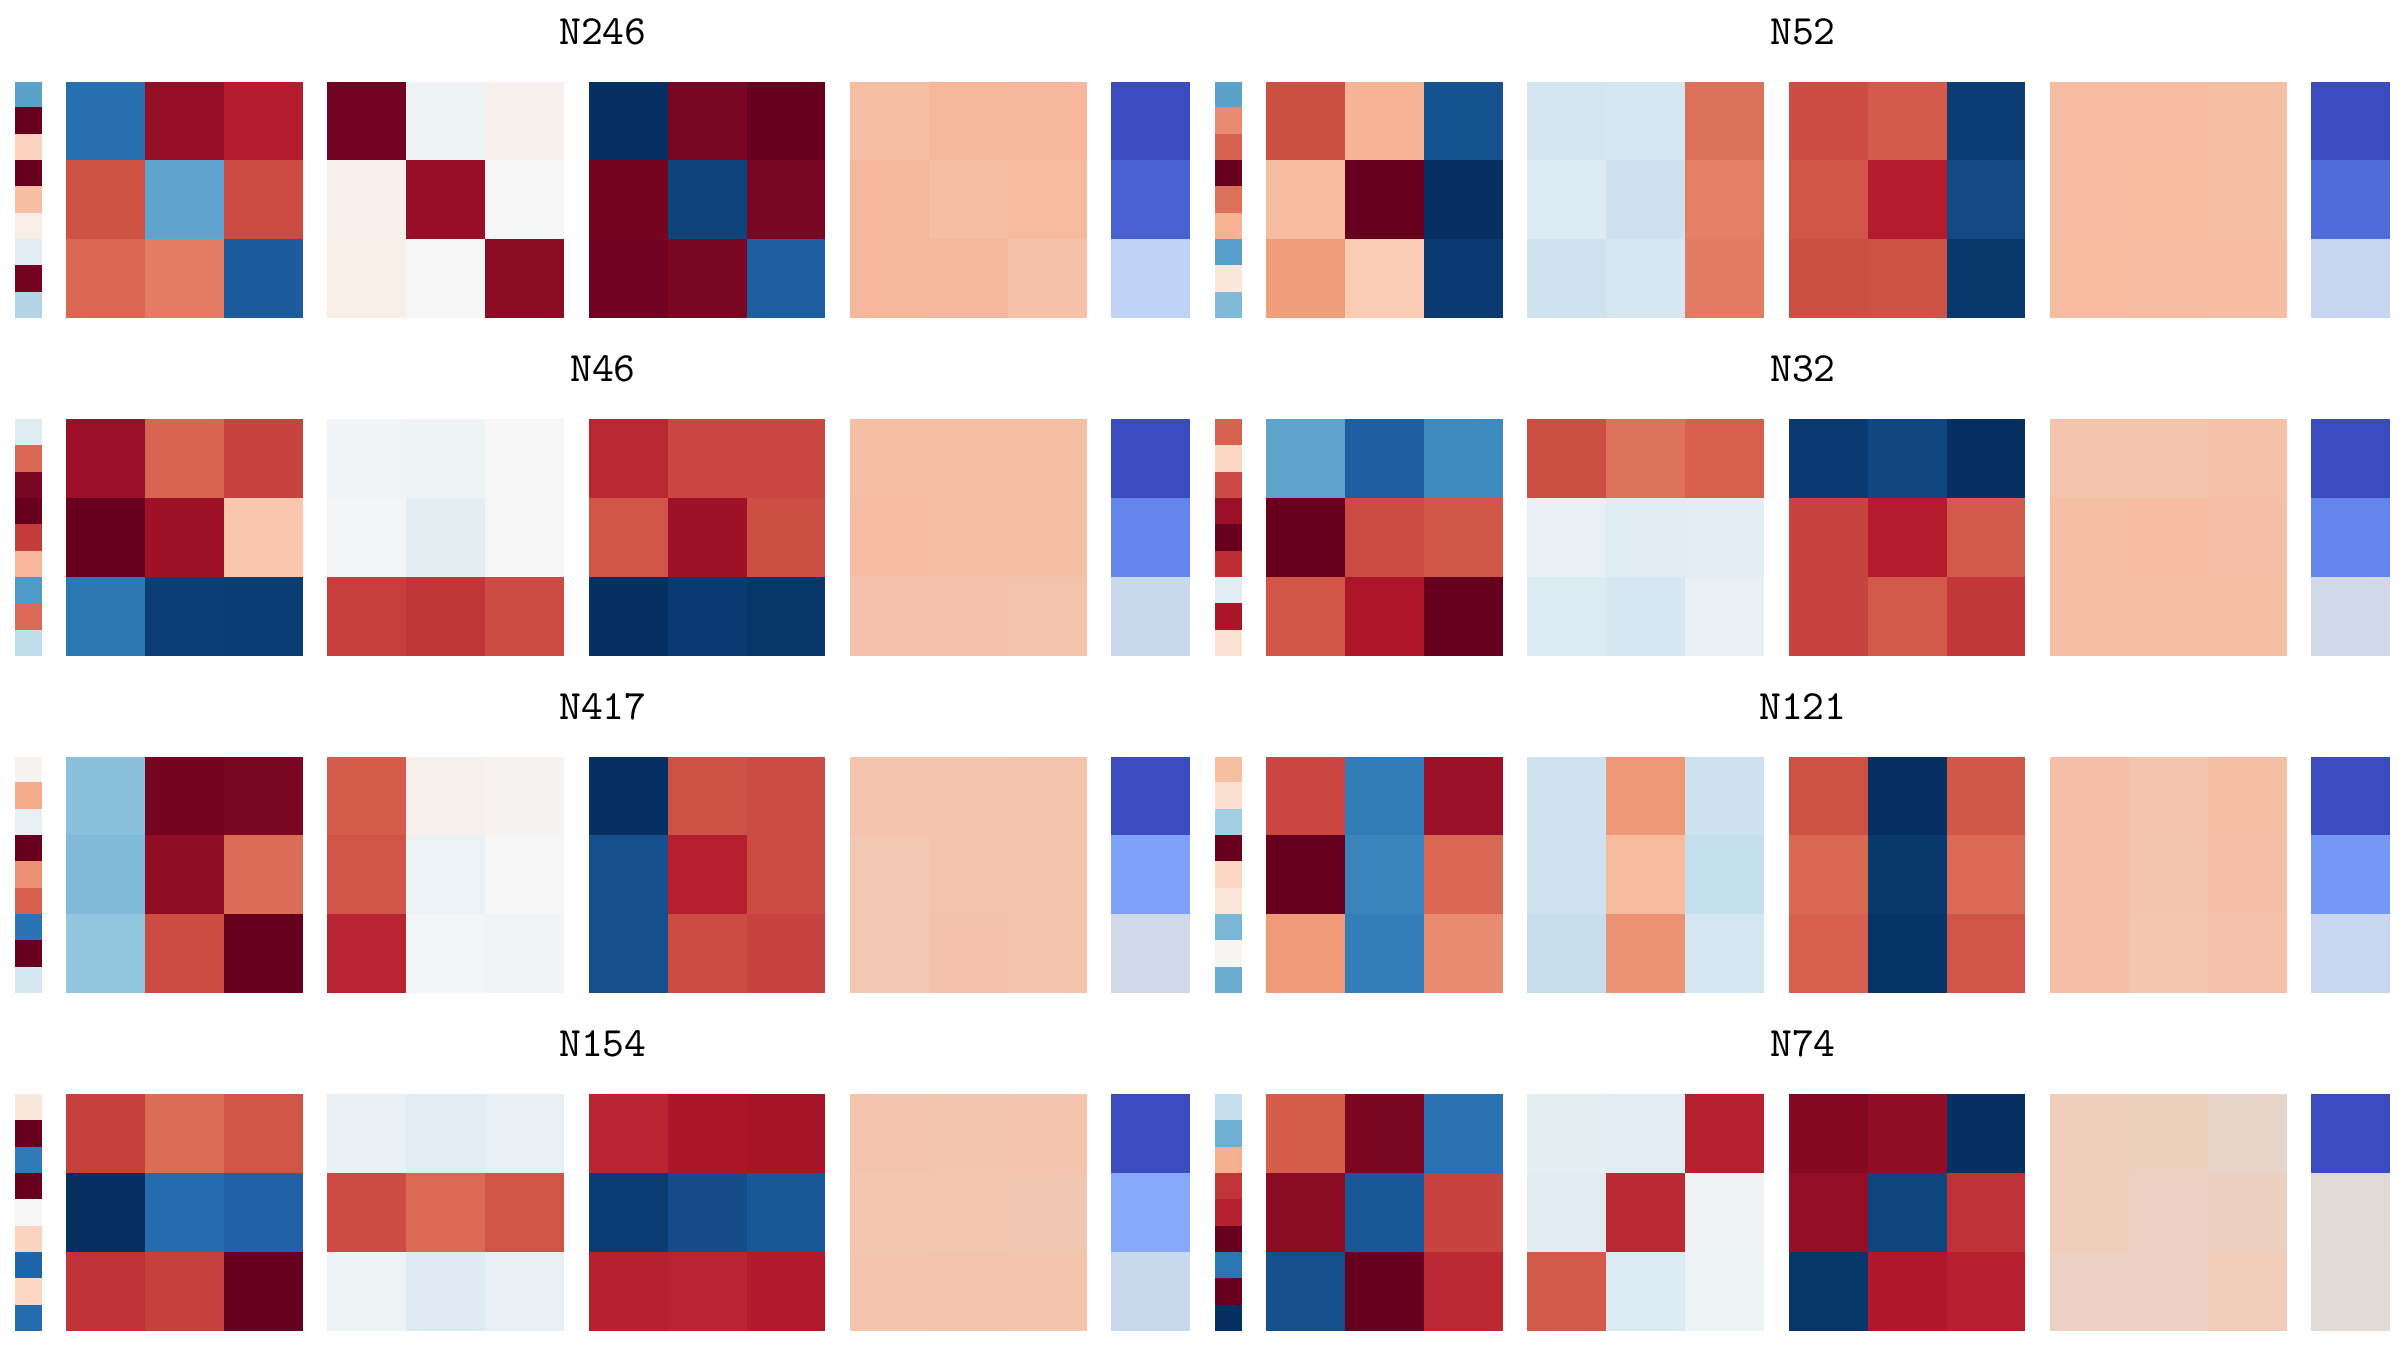
\includegraphics[width=\linewidth]{../out/figs/neuron_category_win_for_x.pdf}
        \caption{Identify wins for \texttt{X}.}
        \label{fig:neurons-x-win}
    \end{subfigure}%
    \hfill
    \begin{subfigure}[b]{0.49\linewidth}
        \includegraphics[width=\linewidth]{../out/figs/neuron_category_win_for_o.pdf}
        \caption{Identify wins for \texttt{O}.}
        \label{fig:neurons-o-win}
    \end{subfigure}
    \begin{subfigure}[b]{0.49\linewidth}
        \includegraphics[width=\linewidth]{../out/figs/neuron_category_move_suppression_single.pdf}
        \caption{Suppress moves already played.}
        \label{fig:neurons-suppress-single}
    \end{subfigure}%
    \hfill
    \begin{subfigure}[b]{0.49\linewidth}
        \includegraphics[width=\linewidth]{../out/figs/neuron_category_anti_win.pdf}
        \caption{Avoid playing moves that lead to wins.}
        \label{fig:neurons-suppress-win}
    \end{subfigure}
    \begin{subfigure}[b]{0.49\linewidth}
        \includegraphics[width=\linewidth]{../out/figs/neuron_category_draw.pdf}
        \caption{Predict draws.}
    \end{subfigure}
    \caption{Categorisation of the top neurons of \ttgpt into the ``rules'' they implement.}
    \label{fig:neuron-categories}
\end{figure}

We can now scale up the visualisation strategy detailed in \cref{fig:neuron-sample} to the rest of the neurons identified in \cref{sec:neurons-that-matter}. Manually inspecting the visualisations reveals that many of neurons are interpretable as they implement certain ``rules'' of the task. The neurons with the most obvious interpretation are the ``\texttt{X} wins'' (\cref{fig:neurons-x-win}) and the ``\texttt{O} wins'' (\cref{fig:neurons-o-win}) neurons. Such neurons react the most strongly to moves via the $\m{W}_{h_1}$ circuit (i.e. moves played by the current player) to determine whether the next token should be a winner's token. It also makes use of the turn number via the $\m{W}_p$ circuit to determine whether the winner should be \texttt{X} for odd-numbered turns, or \texttt{O} for even-numbered turns. Surprisingly, there appears to be exactly 16 of such neurons in \ttgpt, corresponding to the 8 three-in-a-row combinations for each player.

Some other neurons mainly affect the predicted move distributions. For example, I identified ``single move suppression'' neurons that prevent moves that have been played before to be played again on the board (\cref{fig:neurons-suppress-single}). These neurons react to inputs from both the $\m{W}_{h_0}$ and $\m{W}_{h_1}$ circuits which can interpreted as ``no matter who played the move before, the same move cannot be played again''.

Another interest class of neurons are those who affect groups of moves. One outstanding collection of neurons are the ``winning move suppression'' neurons which discourages the probability of playing moves that immediately results in a win. The existence of such neurons matches our intuition as the true task of the model is to predict the game tree distributions, where immediately winning moves have the least number possible continuations. Unlike the ``\texttt{X} wins'' or ``\texttt{O} wins'' neurons that mainly respond to the $\m{W}_{h_1}$ circuit, these neurons reacts strongly to the $\m{W}_{h_0}$ circuit as it needs to attend to the moves played by the opponent. One might argue that the existence of such neurons suggests that \ttgpt has learned to ``think one step ahead'' as the negatives of predicting a winning move only shows after two steps. I tend not to believe in such claim as I observed no other evidence that \ttgpt utilises the min-max nature of the game to make its predictions.

\newpage

\bibliography{references}

\end{document}